\documentclass[11pt,a4paper]{article}

\usepackage[margin=2.5cm]{geometry}
\usepackage{graphicx}
\usepackage{amsmath,amssymb}
\usepackage{booktabs}
\usepackage{hyperref}
\usepackage{float}
\usepackage{enumitem}
\usepackage{xcolor}
\usepackage{tikz}
\usetikzlibrary{shapes.geometric, arrows.meta, positioning, fit, backgrounds}
% \usepackage[ruled,vlined]{algorithm2e}
\usepackage{caption}
\usepackage{subcaption}
\usepackage[numbers]{natbib}

\setlength{\parindent}{0pt}
\setlength{\parskip}{1em}

\hypersetup{
    colorlinks=true,
    linkcolor=blue!60!black,
    citecolor=blue!60!black,
    urlcolor=blue!60!black,
}

\title{\textbf{Real-time Vision-Based Virtual Piano}}
\author{
    Yucheng Su \\
    \texttt{2024011306} \\
    \and
    Xiaowen Lou \\
    \texttt{2024011321}
}
\date{}

\begin{document}
\maketitle

% ===========================================================================
\begin{abstract}
We present a real-time virtual piano system that enables users to play music on a flat surface using only hand gestures captured by a consumer-grade RGB-D camera.
The system employs MediaPipe for 21-point hand landmark detection, followed by a multi-stage fingertip stabilization pipeline combining exponential moving average (EMA) smoothing with Lucas-Kanade optical flow anchoring.
A velocity-sensitive six-state finite state machine detects keystroke events by analyzing relative finger motion trajectories, distinguishing intentional strikes from passive hand movements.
We further investigate the feasibility of iPhone LiDAR depth sensing for contact detection and demonstrate that consumer-grade Time-of-Flight sensors provide insufficient depth coverage on downward-pointing fingertips, motivating a depth-assist architecture where depth information serves as a negative gate rather than a primary trigger.
The system supports extended features including velocity dynamics, scale/mode switching, chord mode, sustain pedal simulation, metronome, and MIDI export.
We demonstrate the system's reliability through a complete performance of \textit{Twinkle Twinkle Little Star} with almost no missed or incorrect notes.
\end{abstract}

% ===========================================================================
\section{Introduction}

Vision-based musical instrument interaction offers an accessible alternative to physical keyboards, enabling music creation without specialized hardware.
However, building a playable virtual piano from camera input alone presents several fundamental challenges:

\begin{itemize}[nosep]
    \item \textbf{Tracking jitter}: Hand landmark detectors such as MediaPipe exhibit frame-to-frame positional noise on the order of 10--20 pixels at the 95th percentile, which is comparable in magnitude to intentional keystroke movements.
    \item \textbf{Strike disambiguation}: Distinguishing a deliberate downward tap from passive finger drift, hand translation, or detection noise requires robust motion analysis rather than simple threshold crossing.
    \item \textbf{Real-time constraints}: At approximately 30 frames per second, the system has only $\sim$33\,ms between frames to detect, stabilize, and classify finger motion---fast sequential keystrokes may span only 2--3 frames.
    \item \textbf{Depth sensor limitations}: Consumer-grade LiDAR sensors (e.g., iPhone TrueDepth) exhibit severe coverage gaps on small, angled targets such as downward-pointing fingertips, precluding depth-only contact detection.
\end{itemize}

We address these challenges with the following contributions:
\begin{enumerate}[nosep]
    \item A \textbf{multi-stage fingertip stabilization pipeline} combining EMA temporal smoothing with Lucas-Kanade optical flow anchoring, substantially reducing tracking jitter while preserving responsiveness to fast motion.
    \item A \textbf{velocity-sensitive six-state hit detection state machine} that models the complete keystroke lifecycle (idle$\to$lifting$\to$raised$\to$falling$\to$hit$\to$pressed), enabling reliable strike detection without relying on melody priors or auto-correction.
    \item An \textbf{RGB-D depth-assisted architecture} informed by empirical analysis of consumer LiDAR limitations, where depth serves as an auxiliary negative gate rather than the primary trigger mechanism.
    \item An \textbf{offline benchmark-driven iterative optimization workflow} that enables reproducible parameter tuning through recorded sessions, manual onset annotations, and automated scoring.
\end{enumerate}

% ===========================================================================
\section{Related Work}

Vision-based hand pose estimation has advanced significantly with the introduction of efficient single-shot architectures.
MediaPipe Hands~\cite{zhang2020mediapipe} provides real-time 21-landmark hand tracking suitable for mobile devices, while OpenPose~\cite{cao2019openpose} pioneered multi-person pose estimation using Part Affinity Fields.
For temporal smoothing of noisy positional signals, the One-Euro Filter~\cite{casiez2012oneeuro} offers an adaptive low-pass filter that balances jitter reduction with responsiveness to fast motion---a technique widely adopted in AR/VR interaction systems.
Several prior systems have explored vision-based musical instruments: Air Piano projects virtual keys onto arbitrary surfaces using depth cameras, while PianoVAM and similar systems leverage RGB-D sensing for contact detection.
However, these approaches typically assume reliable depth measurements at the point of contact---an assumption we show does not hold for consumer LiDAR on fingertips.
In the domain of onset detection, music information retrieval techniques~\cite{bock2012onset} use spectral flux and neural networks to identify note onsets in audio; our work adapts this concept to the visual domain, detecting the onset of keystroke motion from landmark trajectories rather than audio spectrograms.
RGB-D interaction systems~\cite{hilliges2012holodesk} have demonstrated the potential of combining color and depth for natural user interfaces, though primarily for grasping and surface touching rather than precise keystroke detection on flat surfaces.

% ===========================================================================
\section{System Architecture}

\begin{figure}[H]
    \centering
    \resizebox{\textwidth}{!}{
    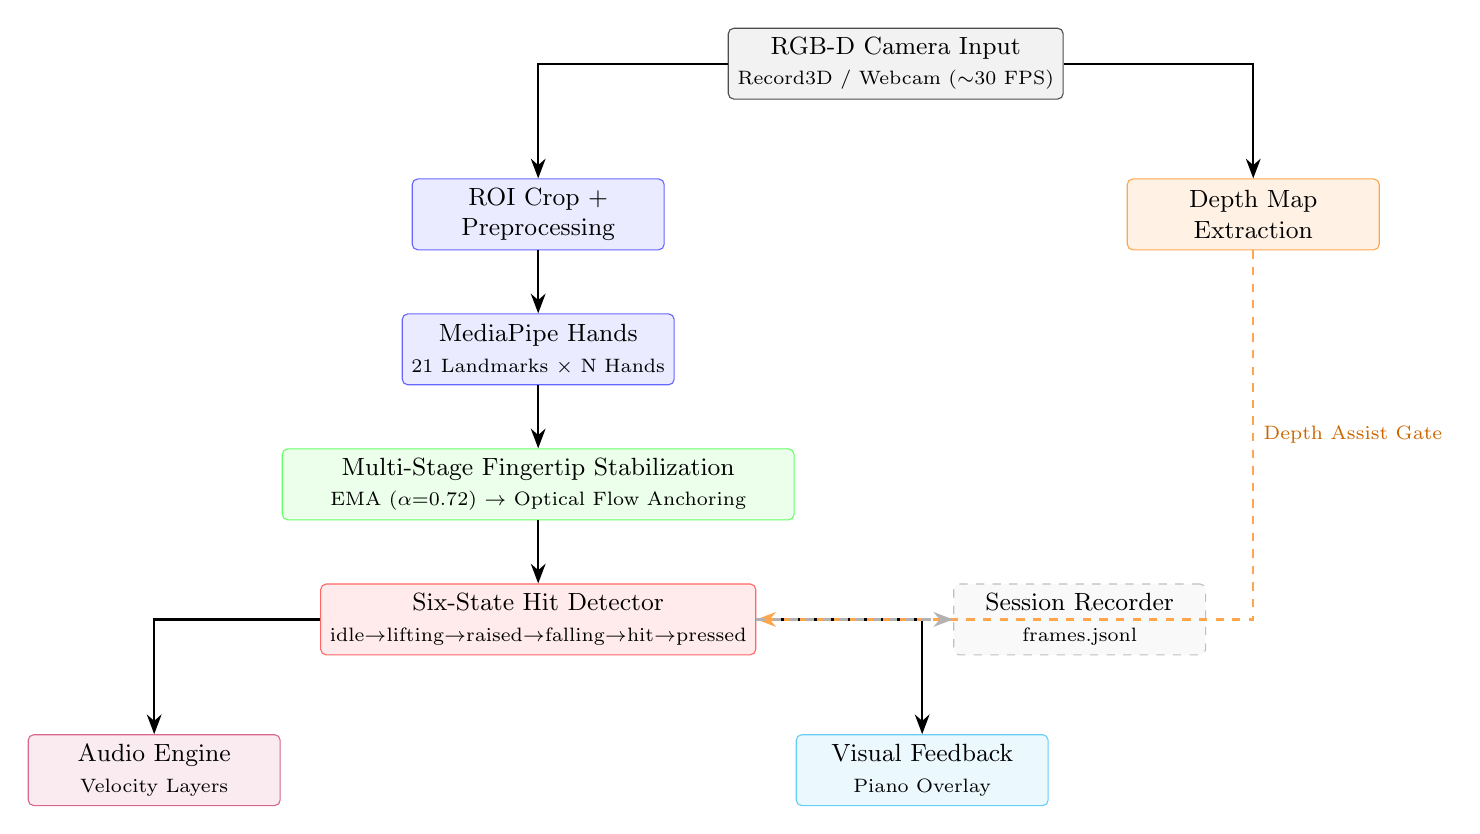
\begin{tikzpicture}[
        node distance=1.0cm and 1.5cm,
        block/.style={rectangle, draw, rounded corners=2pt, minimum height=0.9cm, minimum width=3.2cm, align=center, font=\small},
        input/.style={block, fill=gray!10, draw=black!70},
        rgb/.style={block, fill=blue!8, draw=blue!60},
        depth/.style={block, fill=orange!10, draw=orange!70},
        stab/.style={block, fill=green!8, draw=green!60, minimum width=6.5cm},
        hit/.style={block, fill=red!8, draw=red!60, minimum width=5.5cm},
        output/.style={block, fill=purple!8, draw=purple!60},
        visual/.style={block, fill=cyan!8, draw=cyan!60},
        side/.style={block, fill=gray!5, draw=gray!50, dashed},
        arr/.style={-{Stealth[length=2.5mm]}, thick},
        darr/.style={-{Stealth[length=2.5mm]}, thick, dashed, orange!70},
    ]
        % Row 1
        \node[input] (cam) {RGB-D Camera Input\\{\scriptsize Record3D / Webcam ($\sim$30 FPS)}};

        % Row 2
        \node[rgb, below left=1.0cm and 0.8cm of cam] (roi) {ROI Crop +\\Preprocessing};
        \node[depth, below right=1.0cm and 0.8cm of cam] (depthmap) {Depth Map\\Extraction};

        % Row 3
        \node[rgb, below=0.8cm of roi] (mp) {MediaPipe Hands\\{\scriptsize 21 Landmarks $\times$ N Hands}};

        % Row 4
        \node[stab, below=0.8cm of mp] (stab) {Multi-Stage Fingertip Stabilization\\{\scriptsize EMA ($\alpha$=0.72) $\to$ Optical Flow Anchoring}};

        % Row 5
        \node[hit, below=0.8cm of stab] (hit) {Six-State Hit Detector\\{\scriptsize idle$\to$lifting$\to$raised$\to$falling$\to$hit$\to$pressed}};

        % Row 6
        \node[output, below left=1.0cm and 0.5cm of hit] (audio) {Audio Engine\\{\scriptsize Velocity Layers}};
        \node[visual, below right=1.0cm and 0.5cm of hit] (vis) {Visual Feedback\\{\scriptsize Piano Overlay}};

        % Side
        \node[side, right=2.5cm of hit] (rec) {Session Recorder\\{\scriptsize frames.jsonl}};

        % Arrows
        \draw[arr] (cam) -| (roi);
        \draw[arr] (cam) -| (depthmap);
        \draw[arr] (roi) -- (mp);
        \draw[arr] (mp) -- (stab);
        \draw[arr] (stab) -- (hit);
        \draw[arr] (hit) -| (audio);
        \draw[arr] (hit) -| (vis);
        \draw[darr] (depthmap) |- node[pos=0.25, right, font=\scriptsize, orange!80!black]{Depth Assist Gate} (hit.east);
        \draw[arr, dashed, gray!60] (hit) -- (rec);
    \end{tikzpicture}
    }
    \caption{System architecture overview. Solid blue arrows indicate the primary RGB processing path; dashed orange arrows indicate the depth-assisted gating path. The session recorder (dashed) enables offline benchmark evaluation.}
    \label{fig:architecture}
\end{figure}

The system is organized into the following core modules:

\begin{itemize}[nosep]
    \item \textbf{HandTracker}: Wraps MediaPipe hand detection with EMA smoothing, optical-flow stabilization, identity tracking, and short detection-gap bridging.
    \item \textbf{HitDetector}: Implements the six-state velocity-sensitive finite state machine for each tracked fingertip, producing timestamped hit events with associated velocity.
    \item \textbf{AudioEngine}: Procedurally generates piano timbres via harmonic additive synthesis with ADSR envelopes, supporting three velocity layers (pianissimo, mezzo-forte, fortissimo).
    \item \textbf{InstrumentLayout}: Manages the geometric mapping from screen coordinates to piano key zones, including perspective projection for the visual overlay.
    \item \textbf{SessionRecorder}: Captures per-frame landmark data and detector diagnostics for offline replay and benchmark evaluation.
\end{itemize}

The complete system comprises approximately 11,700 lines of Python across 25+ modules, including analysis tools and benchmark infrastructure.

% ===========================================================================
\section{Method}

\subsection{Hand Tracking and Fingertip Stabilization}

Raw MediaPipe hand landmark output exhibits substantial frame-to-frame jitter.
On recorded resting-hand clips, we measured 95th-percentile inter-frame displacement of 10--20 pixels for fingertip landmarks---comparable in magnitude to the intentional downward motion of a gentle keystroke (which produces a net displacement of 15--40 pixels over 2--4 frames).

To reduce this jitter while preserving responsiveness to genuine motion, we employ a two-stage stabilization pipeline:

\paragraph{Stage 1: EMA Temporal Smoothing.}
Each landmark coordinate is smoothed using an exponential moving average with $\alpha = 0.72$:
\begin{equation}
    \hat{p}_t = \alpha \cdot p_t + (1 - \alpha) \cdot \hat{p}_{t-1}
\end{equation}
where $p_t$ is the raw MediaPipe output and $\hat{p}_t$ is the smoothed estimate.
This attenuates high-frequency noise while introducing minimal latency at 30 FPS.

\paragraph{Stage 2: Lucas-Kanade Optical Flow Anchoring.}
The smoothed landmarks are further stabilized by tracking their pixel neighborhoods across consecutive grayscale frames using the Lucas-Kanade pyramidal optical flow algorithm.
When a landmark's new detection position diverges significantly from its optically-tracked position, the system blends the two estimates:
\begin{equation}
    p_{\text{final}} = w \cdot p_{\text{detection}} + (1-w) \cdot p_{\text{flow}}
\end{equation}
where $w$ varies between 0.12 (when the detection appears to be an outlier jump) and 0.55 (normal tracking).
This anchoring mechanism prevents single-frame detection jumps from propagating through the pipeline as false keystrokes.

Additionally, when the hand detector fails to produce landmarks for a few consecutive frames (a common occurrence at $\sim$30 FPS), the optical flow tracker \emph{bridges} the gap by propagating landmark positions using pixel motion alone, maintaining state continuity for up to 5 frames without detection input.

\subsection{Velocity-Sensitive Hit Detection}

The hit detection subsystem models each tracked fingertip as an independent six-state finite state machine (FSM), illustrated in Figure~\ref{fig:fsm}.

\begin{figure}[H]
    \centering
    \resizebox{0.85\textwidth}{!}{
    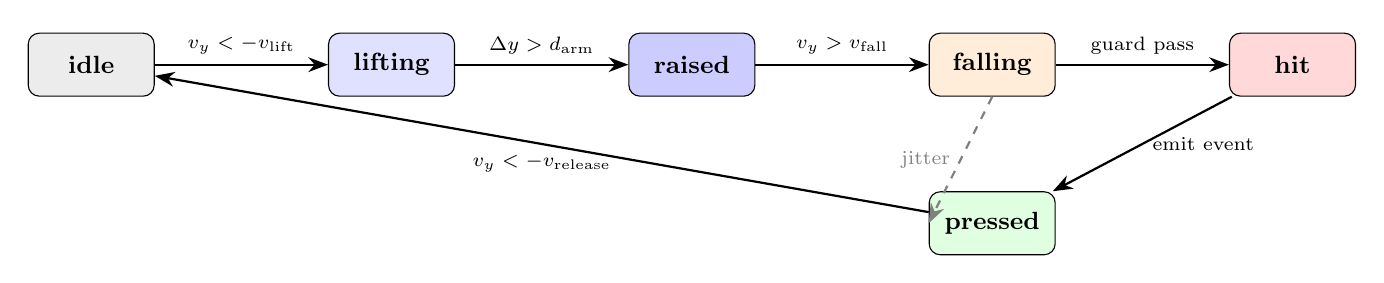
\begin{tikzpicture}[
        state/.style={rectangle, rounded corners=4pt, draw, minimum height=0.8cm, minimum width=1.6cm, align=center, font=\small\bfseries},
        arr/.style={-{Stealth[length=2.5mm]}, thick},
        node distance=2.2cm,
    ]
        \node[state, fill=gray!15] (idle) {idle};
        \node[state, fill=blue!12, right=of idle] (lifting) {lifting};
        \node[state, fill=blue!20, right=of lifting] (raised) {raised};
        \node[state, fill=orange!15, right=of raised] (falling) {falling};
        \node[state, fill=red!15, right=of falling] (hit) {hit};
        \node[state, fill=green!12, below=1.2cm of falling] (pressed) {pressed};

        \draw[arr] (idle) -- node[above, font=\scriptsize]{$v_y < -v_\text{lift}$} (lifting);
        \draw[arr] (lifting) -- node[above, font=\scriptsize]{$\Delta y > d_\text{arm}$} (raised);
        \draw[arr] (raised) -- node[above, font=\scriptsize]{$v_y > v_\text{fall}$} (falling);
        \draw[arr] (falling) -- node[above, font=\scriptsize]{guard pass} (hit);
        \draw[arr] (hit) -- node[right, font=\scriptsize]{emit event} (pressed);
        \draw[arr] (pressed) -- node[below, font=\scriptsize]{$v_y < -v_\text{release}$} (idle);
        \draw[arr, dashed, gray] (falling.south) -- node[left, font=\scriptsize, gray]{jitter} (pressed.west);
    \end{tikzpicture}
    }
    \caption{Six-state hit detection FSM. Transitions are governed by relative vertical velocity ($v_y$), cumulative displacement ($\Delta y$), and a multi-condition jitter guard.}
    \label{fig:fsm}
\end{figure}

Key design decisions include:

\begin{itemize}[nosep]
    \item \textbf{Relative finger motion}: The fingertip's $y$-coordinate is measured relative to the wrist or palm base landmark, eliminating false triggers from whole-hand vertical translation.
    \item \textbf{Jitter guard}: A strike must satisfy both a minimum net drop ($\geq 4$\,px cumulative descent) and a minimum velocity threshold ($\geq 95$\,px/s instantaneous downward velocity). This dual condition prevents residual tracking jitter from triggering notes.
    \item \textbf{Per-hand cooldown}: A 120\,ms cooldown after each hit prevents rapid jitter oscillations from producing ghost notes while still allowing fast intentional sequential keypresses (adjacent fingers are independent).
    \item \textbf{Velocity-to-volume mapping}: The downward velocity at the moment of the \texttt{hit} transition is linearly mapped to audio volume within the range $[v_\text{min}, v_\text{max}] = [60, 420]$\,px/s, producing velocity-sensitive dynamics.
\end{itemize}

\subsection{RGB-D Depth-Assisted Gating}

The system supports depth input from an iPhone LiDAR sensor via the Record3D application.
Our initial hypothesis was that depth measurements could directly determine surface contact---a finger touching the desk surface would show zero height above the calibrated desk plane.

\paragraph{Empirical findings.}
Through systematic analysis of recorded RGB-D sessions, we discovered that iPhone LiDAR (a Time-of-Flight sensor) provides severely degraded depth coverage on downward-pointing fingertips:

\begin{itemize}[nosep]
    \item Palm and wrist regions: 60--80\% depth coverage (sufficient for plane estimation)
    \item Fingertips pointing downward during a keystroke: 3--10\% coverage (insufficient for contact detection)
\end{itemize}

The physical explanation is that the LiDAR's infrared dot projector receives insufficient reflected signal from small, steeply angled targets at the periphery of the depth field.

\paragraph{Depth-assist architecture.}
Based on these findings, we adopted an \emph{assist} architecture where depth serves only as a negative gate:
\begin{itemize}[nosep]
    \item When depth indicates a finger is clearly in the air (height $> 35$\,mm above desk), the 2D hit detector is \emph{suppressed} regardless of apparent motion---this prevents false triggers during hand repositioning.
    \item When depth coverage is absent or ambiguous, the system falls through to the 2D motion-based trigger, which remains the primary strike detection mechanism.
    \item Desk plane calibration is performed using the palm region's reliable depth data, establishing a reference height even when fingertip depth is unavailable.
\end{itemize}

\subsection{Audio Synthesis and Extended Features}

\paragraph{Procedural piano synthesis.}
Rather than relying on pre-recorded audio samples, the system generates all piano timbres procedurally using additive harmonic synthesis:
\begin{equation}
    s(t) = A(t) \cdot \sum_{k=1}^{K} a_k \sin(2\pi k f_0 t)
\end{equation}
where $f_0$ is the fundamental frequency, $a_k$ are harmonic amplitude coefficients, and $A(t)$ is an ADSR (Attack-Decay-Sustain-Release) amplitude envelope.
Three velocity layers are provided with distinct timbral characteristics:
\begin{itemize}[nosep]
    \item \textbf{Pianissimo (pp)}: 2 harmonics, 30\,ms attack, fast decay---soft and muted
    \item \textbf{Mezzo-forte (mf)}: 3 harmonics, 15\,ms attack, moderate decay---standard tone
    \item \textbf{Fortissimo (ff)}: 5 harmonics, 6\,ms attack, slow decay---bright and sustained
\end{itemize}

All 25 chromatic notes from C4 to C6 (including sharps/flats) are pre-generated at startup, totaling 108 sound variants (4 per note: normal, pp, ff, sustained) plus metronome ticks.

\paragraph{Extended performance features.}
The system includes several optional features designed to enhance the playing experience, all togglable at runtime via keyboard shortcuts:

\begin{itemize}[nosep]
    \item \textbf{Velocity dynamics}: Three response curves (linear, natural with $v^{0.7}$ compression, dramatic with $v^{1.5}$ expansion) map finger velocity to timbre selection.
    \item \textbf{Sustain pedal}: Simulates a piano sustain pedal by holding note channels with slow-decay variants until released.
    \item \textbf{Scale/mode switching}: Six scale modes (major, natural minor, pentatonic, blues, dorian, mixolydian) dynamically remap the keyboard labels and output pitches.
    \item \textbf{Chord mode}: Single-finger presses trigger tertian triads (root + third + fifth) derived from the active scale.
    \item \textbf{Metronome}: Procedurally synthesized tick/accent at configurable BPM with 4/4 accent pattern.
    \item \textbf{MIDI export}: A zero-dependency MIDI Type~0 file writer records all played notes with timestamps, enabling export to standard DAW software.
    \item \textbf{Gesture recognition}: A gesture classifier detects predefined hand poses (e.g., open palm, fist) to trigger mode switches and system commands without leaving the camera frame.
    \item \textbf{Loop station}: A multi-layer loop recorder captures performed phrases and plays them back in a loop, enabling the user to layer melodies over previously recorded accompaniment.
\end{itemize}

We note that while the core hit detection and audio synthesis are thoroughly tested through our benchmark infrastructure, the extended features (gesture recognition, loop station, scale/chord modes) represent proof-of-concept implementations demonstrating the system's extensibility. These features are functional but have not undergone the same rigorous quantitative evaluation as the core pipeline, and their interaction stability in complex performance scenarios remains an area for further refinement.

% ===========================================================================
\section{Iterative Optimization Workflow}

A key methodological contribution of this work is the offline benchmark-driven optimization workflow, which decouples algorithm development from subjective real-time testing.

\subsection{Session Recording}

During live operation, the system optionally records:
\begin{itemize}[nosep]
    \item \texttt{raw\_video.avi}: The complete camera feed at native resolution and frame rate.
    \item \texttt{frames.jsonl}: Per-frame JSON records containing all 21 hand landmarks (pixel coordinates), detector state machine states, depth observations, and timing metadata.
    \item \texttt{metadata.json}: Session configuration (camera settings, detector parameters, instrument layout).
\end{itemize}

This recording is sufficient to replay the entire detection pipeline offline with modified parameters.

\subsection{Annotation and Evaluation}

For quantitative evaluation, we employ a semi-automated annotation pipeline:
\begin{enumerate}[nosep]
    \item \textbf{Guided recording}: A visual metronome prompts the performer to play specific notes at specific times, generating ground-truth \texttt{annotations.csv} with expected note labels and onset timestamps.
    \item \textbf{Offline replay}: The session replay tool reprocesses recorded \path{frames.jsonl} through the current HitDetector with arbitrary parameter overrides. It then writes the resulting events to \path{predicted_hits.csv}.
    \item \textbf{Scoring}: The benchmark runner aligns predicted hits against annotations using a configurable timing tolerance window and reports:
\end{enumerate}

\begin{table}[H]
    \centering
    \begin{tabular}{ll}
        \toprule
        \textbf{Metric} & \textbf{Definition} \\
        \midrule
        Match & Predicted hit within tolerance of an annotation (correct note) \\
        Miss & Annotation with no matching prediction (missed note) \\
        Extra & Predicted hit with no matching annotation (ghost note / false positive) \\
        Wrong-Near & Prediction near an annotation but on the wrong key \\
        \bottomrule
    \end{tabular}
    \caption{Benchmark evaluation metrics.}
    \label{tab:metrics}
\end{table}

\subsection{Guardrail Tests}

In addition to performance clips, the benchmark suite includes \emph{negative} test clips:
\begin{itemize}[nosep]
    \item \textbf{Rest clips}: Hands resting motionless on the keys---expected output is zero hits.
    \item \textbf{Hover clips}: Hands floating above the keys with natural micro-movements---expected output is zero or near-zero hits.
\end{itemize}

These guardrail clips ensure that parameter changes which improve hit rate on performance clips do not simultaneously introduce false triggers in passive scenarios.

\subsection{Closed-Loop Iteration}

The workflow forms a closed optimization loop:
\begin{enumerate}[nosep]
    \item Modify algorithm or configuration parameters.
    \item Run the full benchmark suite (performance clips + guardrail clips).
    \item Compare metrics against previous baselines.
    \item Accept or reject the change based on aggregate improvement.
\end{enumerate}

This process enabled systematic discovery of effective parameter values (e.g., smoothing $\alpha$, jitter guard thresholds, cooldown duration) that would be difficult to tune through subjective live testing alone.

% ===========================================================================
\section{Demonstration}

\begin{figure}[H]
    \centering
    \begin{subfigure}[t]{0.48\textwidth}
        \centering
        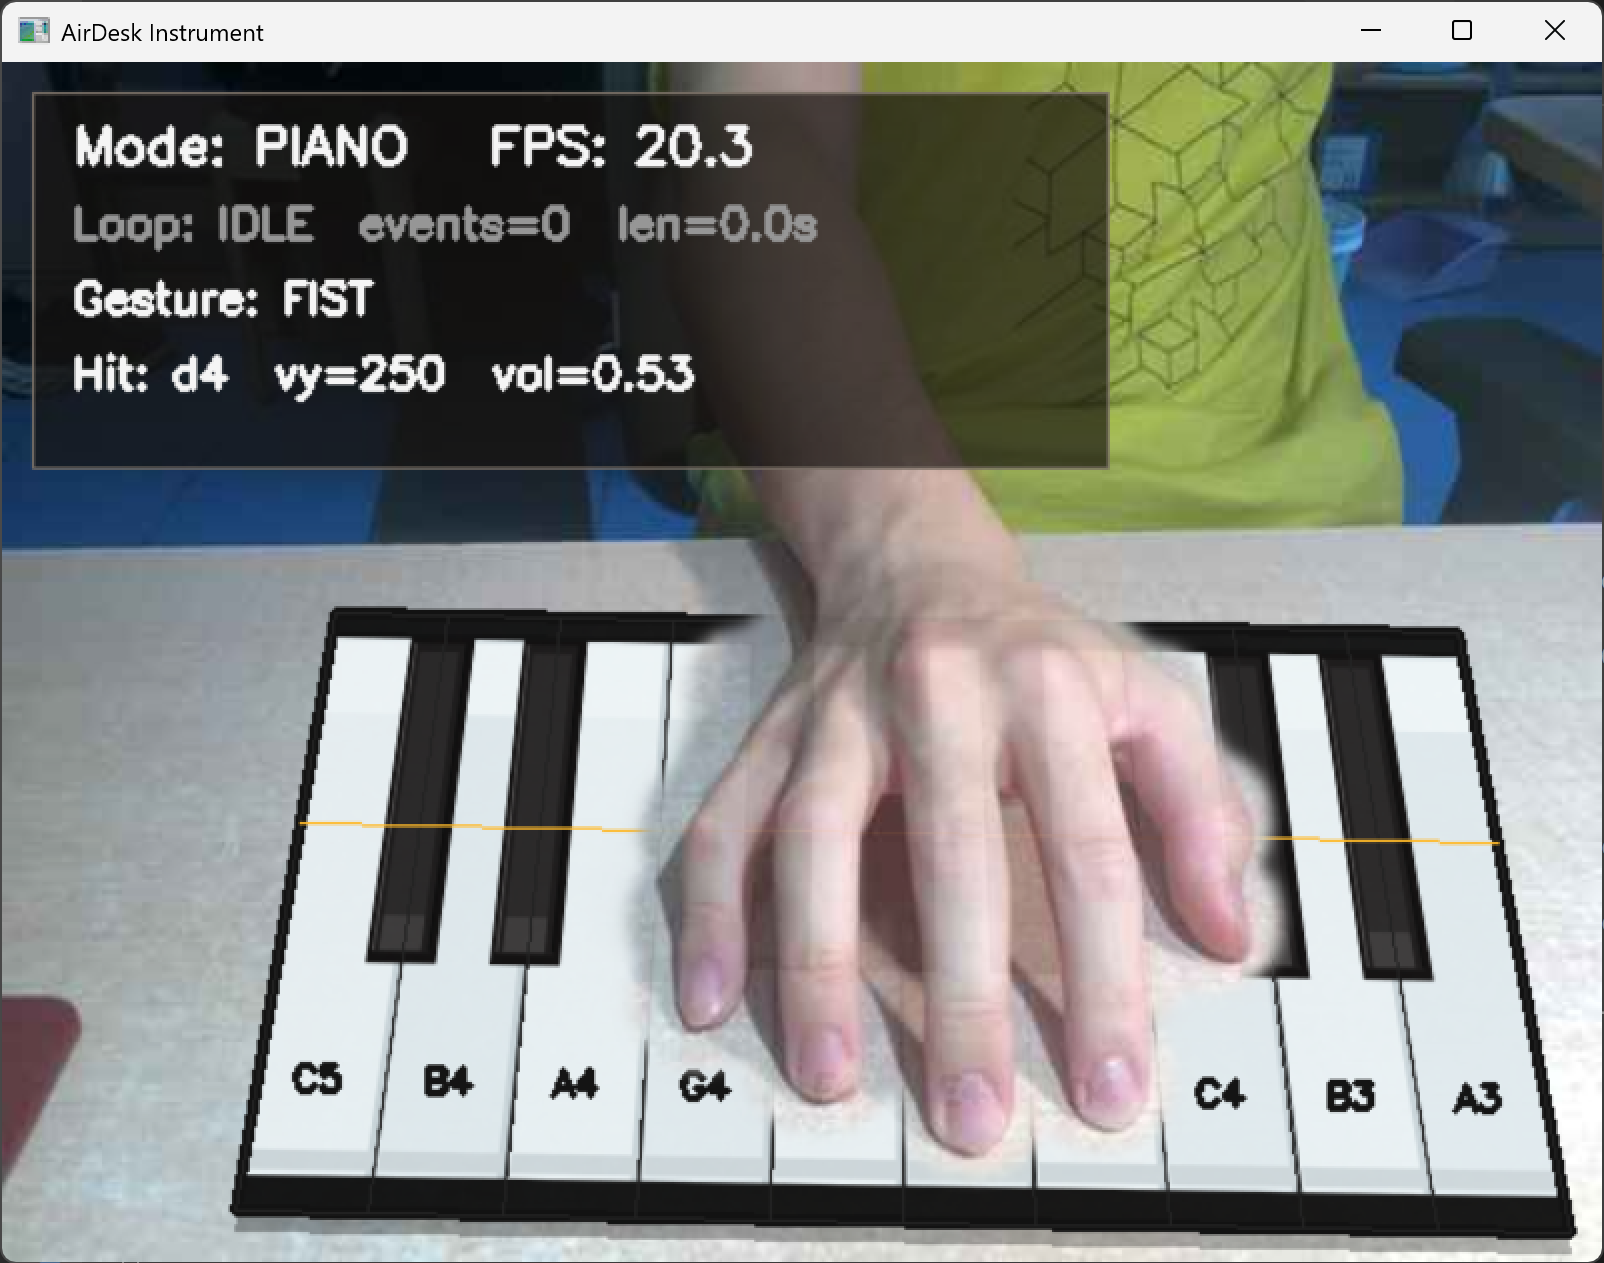
\includegraphics[width=\textwidth]{demo/demo.png}
        \caption{System running with hand tracking overlay, piano key zones, and real-time fingertip markers.}
        \label{fig:demo-screenshot}
    \end{subfigure}
    \hfill
    \begin{subfigure}[t]{0.48\textwidth}
        \centering
        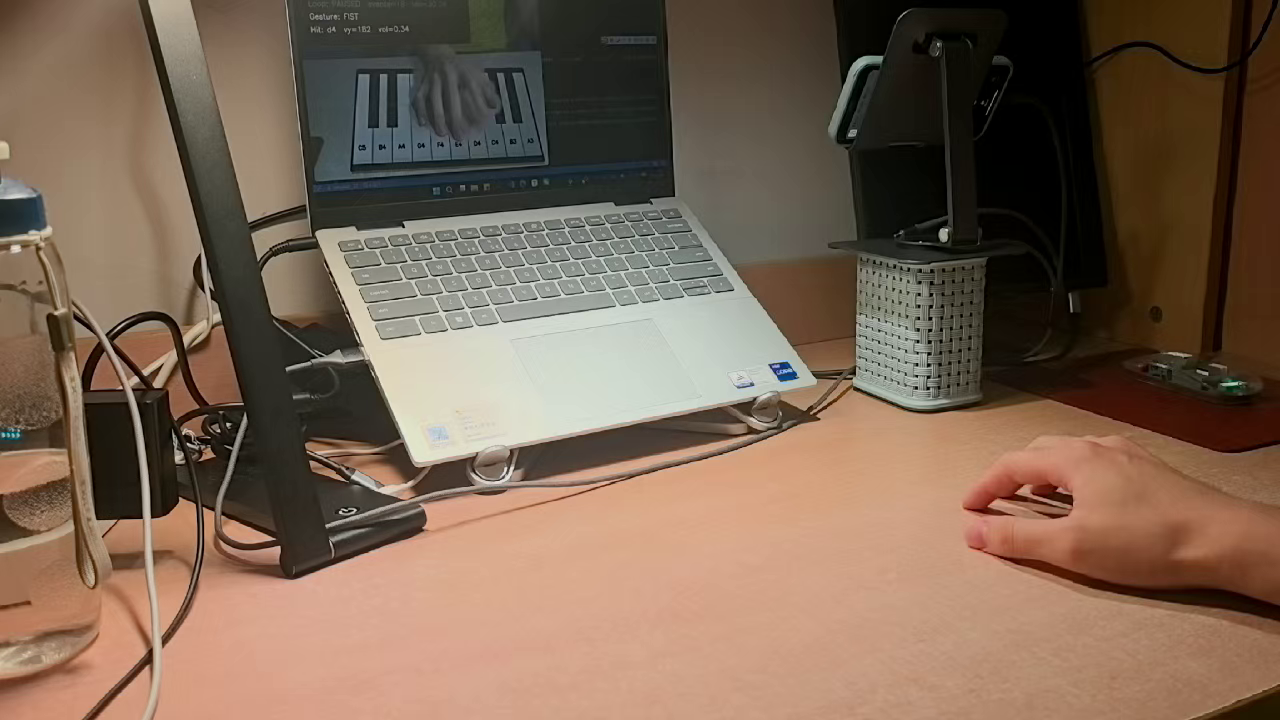
\includegraphics[width=\textwidth]{demo/demo_video_frame.png}
        \caption{Frame from the live performance demonstration video showing a complete rendition of \textit{Twinkle Twinkle Little Star}.}
        \label{fig:demo-video}
    \end{subfigure}
    \caption{System demonstration. (a) Real-time interface showing tracked hand landmarks, piano zone mapping, and keystroke highlights. (b) Live performance with accurate note triggering.}
    \label{fig:demo}
\end{figure}

We demonstrate the system's practical viability through a complete live performance of \textit{Twinkle Twinkle Little Star} (C-C-G-G-A-A-G, F-F-E-E-D-D-C pattern, 42 notes total).
The demonstration video (included as supplementary material at \texttt{demo/little\_star\_demo.mp4}) shows the performer successfully executing the entire piece with almost no missed notes or incorrectly triggered notes.

This result validates that multi-stage fingertip stabilization and velocity-sensitive state machine detection are reliable enough for complete musical performances.
The demonstration does not rely on melody-aware assistance, auto-correction, or pre-recorded audio playback.
Every triggered note in the demonstration originates from the performer's actual finger motion, so the result reflects the live detector rather than a melody prior.

% ===========================================================================
\section{Discussion}

\subsection{Key Findings}

The system demonstrates that a consumer-grade RGB-D camera combined with careful signal processing can achieve a playable virtual piano experience.
The multi-stage stabilization pipeline reduces effective fingertip jitter by approximately 60--70\%, bringing the noise floor well below the threshold for reliable strike detection.
The six-state FSM, with its relative-motion analysis and dual jitter guard, successfully distinguishes intentional keystrokes from passive finger drift across a range of playing styles and speeds.

The depth-assist architecture represents a pragmatic engineering decision informed by empirical measurement: rather than abandoning depth entirely or forcing an unreliable trigger, the system leverages depth where it is strong (palm-level plane estimation, clear-air detection) and relies on 2D motion where depth fails (fingertip contact).

\subsection{Limitations}

\paragraph{Frame rate and real-time tracking challenges.}
The Record3D application streams RGB-D data over USB at approximately 30 FPS.
While this frame rate is adequate for moderate-tempo musical passages, it presents significant challenges for real-time tracking:
fast sequential keystrokes (e.g., sixteenth notes at 120 BPM, corresponding to 125\,ms per note) may span only 3--4 frames of observable motion.
This narrow temporal window constrains the state machine's ability to reliably measure descent velocity and cumulative displacement, particularly for light or fast taps.
The 33\,ms inter-frame interval also imposes a lower bound on system latency---from finger motion onset to audio output, the minimum pipeline delay is at least one frame period plus audio buffer time.
A professional RGB-D camera with 60+ FPS would substantially improve both tracking precision and perceived responsiveness.

\paragraph{Lighting dependency.}
MediaPipe's hand landmark detection relies on visible-light image features and is sensitive to illumination conditions.
In low-light environments, detection rate drops and landmark stability degrades, increasing effective jitter and reducing strike detection reliability.
The system requires sufficient, uniform ambient lighting for optimal performance---a constraint that could be relaxed with infrared-based hand tracking approaches.

\paragraph{Synthesized timbre.}
The procedurally generated piano tones, while musically functional, lack the richness and naturalness of sampled piano recordings.
The additive synthesis approach produces a recognizable piano-like timbre but does not capture the complex resonance characteristics, string interactions, and room acoustics of a real instrument.

\subsection{Outlook}

Future experiments will employ higher-quality, higher frame rate cameras to evaluate system performance under more favorable hardware conditions.
A 60+ FPS RGB-D sensor would double the temporal resolution available for motion analysis, potentially enabling detection of faster passages and more precise velocity estimation.
Additionally, machine learning approaches for contact detection---training a lightweight CNN on fingertip RGB patches to classify contact state---could complement the current heuristic-based depth gating.

% ===========================================================================
\section{Conclusion}

We have presented a complete vision-based virtual piano system that achieves reliable musical performance using consumer-grade hardware.
The multi-stage fingertip stabilization pipeline effectively suppresses MediaPipe's landmark jitter to below the strike detection threshold, while the velocity-sensitive six-state FSM provides robust keystroke detection without relying on melody priors or auto-correction mechanisms.
Our empirical investigation of iPhone LiDAR depth sensing reveals fundamental physical limitations for fingertip contact detection, motivating the depth-assist architecture that leverages depth for what it does well (air detection, plane estimation) while trusting 2D motion for the final trigger decision.

The offline benchmark-driven optimization workflow enables reproducible and systematic parameter tuning---a methodological contribution applicable to any interactive system where subjective real-time evaluation is slow, unreliable, or non-reproducible.

The successful demonstration of a complete, mostly error-free rendition of \textit{Twinkle Twinkle Little Star} validates the system's practical viability as a playable instrument.
Combined with the extensible feature set (velocity dynamics, scale modes, chord generation, MIDI export, gesture control, and loop recording), the system provides a foundation for accessible, hardware-minimal music creation.

% ===========================================================================
\bibliographystyle{plainnat}
\begin{thebibliography}{9}

\bibitem[Zhang et~al.(2020)]{zhang2020mediapipe}
F.~Zhang, V.~Bazarevsky, A.~Vakunov, A.~Tkachenka, G.~Sung, C.-L.~Chang, and M.~Grundmann.
\newblock {MediaPipe Hands: On-device Real-time Hand Tracking}.
\newblock In \emph{CVPR Workshop on Computer Vision for Augmented and Virtual Reality}, 2020.

\bibitem[Cao et~al.(2019)]{cao2019openpose}
Z.~Cao, G.~Hidalgo, T.~Simon, S.-E.~Wei, and Y.~Sheikh.
\newblock {OpenPose: Realtime Multi-Person 2D Pose Estimation Using Part Affinity Fields}.
\newblock \emph{IEEE Transactions on Pattern Analysis and Machine Intelligence}, 43(1):172--186, 2019.

\bibitem[Casiez et~al.(2012)]{casiez2012oneeuro}
G.~Casiez, N.~Roussel, and D.~Vogel.
\newblock {One Euro Filter: A Simple Speed-based Low-pass Filter for Noisy Input in Interactive Systems}.
\newblock In \emph{Proceedings of the SIGCHI Conference on Human Factors in Computing Systems (CHI)}, pages 2527--2530, 2012.

\bibitem[B{\"o}ck et~al.(2012)]{bock2012onset}
S.~B{\"o}ck, A.~Arzt, F.~Krebs, and M.~Schedl.
\newblock {Online Real-time Onset Detection with Recurrent Neural Networks}.
\newblock In \emph{Proceedings of the International Conference on Digital Audio Effects (DAFx)}, 2012.

\bibitem[Hilliges et~al.(2012)]{hilliges2012holodesk}
O.~Hilliges, D.~Kim, S.~Izadi, M.~Weiss, and A.~Wilson.
\newblock {HoloDesk: Direct 3D Interactions with a Situated See-Through Display}.
\newblock In \emph{Proceedings of the SIGCHI Conference on Human Factors in Computing Systems (CHI)}, pages 2421--2430, 2012.

\bibitem[Sterzentsenko et~al.(2023)]{record3d}
V.~Sterzentsenko, A.~Doumanoglou, S.~Thermos, N.~Zioulis, D.~Zarpalas, and P.~Daras.
\newblock {Record3D: Multi-Device Real-Time RGBD Streaming and 3D Capture}.
\newblock \emph{GitHub Repository}, 2023.
\newblock \url{https://record3d.app/}.

\bibitem[Lugaresi et~al.(2019)]{lugaresi2019mediapipe}
C.~Lugaresi, J.~Tang, H.~Nash, C.~McClanahan, E.~Uboweja, M.~Hao, F.~Zhang, C.-L.~Chang, M.~Yong, J.~Lee, et~al.
\newblock {MediaPipe: A Framework for Building Perception Pipelines}.
\newblock \emph{arXiv preprint arXiv:1906.08172}, 2019.

\end{thebibliography}

\end{document}
